\documentclass[12pt]{article}

\usepackage{amsmath}
\usepackage{hyperref}
\usepackage{graphicx}
\usepackage{float}
\usepackage{caption}
\usepackage{listings}
\usepackage{xcolor}
\usepackage{pgfplots}
\usepackage{tikz}
\usetikzlibrary{snakes}
\usepackage{rotating}
\usetikzlibrary{arrows.meta, shapes}

% Define colors
\colorlet{punct}{red!60!black}
\definecolor{background}{RGB}{240, 248, 255} % Pale Blue
\definecolor{delim}{RGB}{20,105,176}
\colorlet{numb}{magenta!60!black}

% Define JSON language
\lstdefinelanguage{json}{
    basicstyle=\ttfamily\footnotesize\color{black},
    basicstyle=\ttfamily\footnotesize\color{black},
    numbers=left,
    numberstyle=\scriptsize,
    stepnumber=1,
    numbersep=8pt,
    showstringspaces=false,
    breaklines=true,
    frame=lines,
    backgroundcolor=\color{background},
    literate=
     *{0}{{{\color{numb}0}}}{1}
      {1}{{{\color{numb}1}}}{1}
      {2}{{{\color{numb}2}}}{1}
      {3}{{{\color{numb}3}}}{1}
      {4}{{{\color{numb}4}}}{1}
      {5}{{{\color{numb}5}}}{1}
      {6}{{{\color{numb}6}}}{1}
      {7}{{{\color{numb}7}}}{1}
      {8}{{{\color{numb}8}}}{1}
      {9}{{{\color{numb}9}}}{1}
      {:}{{{\color{punct}{:}}}}{1}
      {,}{{{\color{punct}{,}}}}{1}
      {\{}{{{\color{delim}{\{}}}}{1}
      {\}}{{{\color{delim}{\}}}}}{1}
      {[}{{{\color{delim}{[}}}}{1}
      {]}{{{\color{delim}{]}}}}{1},
}



\setlength{\parskip}{1em}

\lstset{frame=single, showstringspaces=false, columns=fixed, basicstyle={\ttfamily}, commentstyle={\it}, numbers=left, tabsize=4}

\definecolor{codebackground}{RGB}{240, 248, 255}
\definecolor{codecomment}{RGB}{106,153,85}
\definecolor{codekeyword}{RGB}{30,30,255}
\definecolor{codestring}{RGB}{163,21,21}
\definecolor{codenumber}{RGB}{100,100,100}

\lstdefinestyle{modernstyle}{
    backgroundcolor=\color{codebackground},
    commentstyle=\color{codecomment},
    keywordstyle=\color{codekeyword},
    numberstyle=\tiny\color{codenumber},
    stringstyle=\color{codestring},
    basicstyle=\ttfamily\footnotesize\color{black},
    breakatwhitespace=false,
    breaklines=true,
    captionpos=b,
    keepspaces=true,
    numbers=left,
    numbersep=5pt,
    showspaces=false,
    showstringspaces=false,
    showtabs=false,
    tabsize=4
}


\lstset{style=modernstyle}

\begin{document}

\begin{titlepage}
\centering
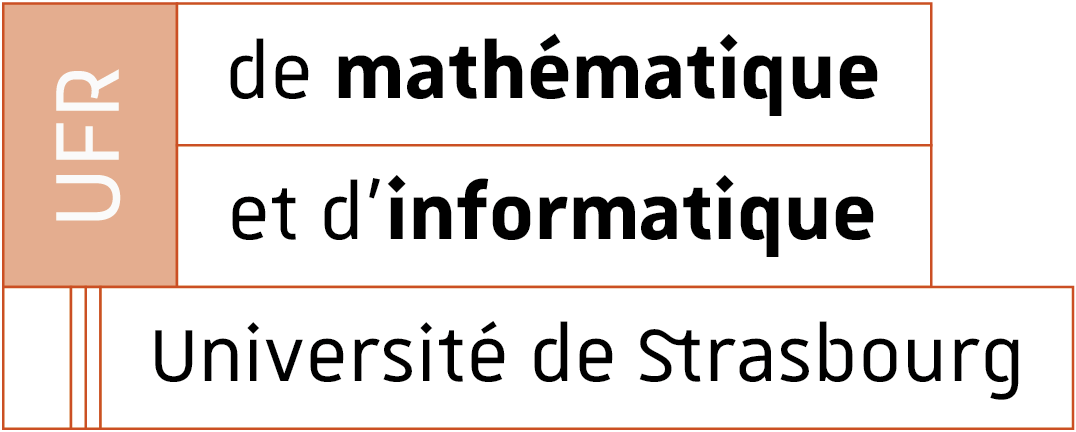
\includegraphics[width=0.5\textwidth]{images/logo_ufr.png}\par\vspace{1cm}
\vspace{1.5cm}
{\huge\bfseries ExaMA WP1 - Vegetation\par}
\vspace{2cm}
{\Large Giulio Carpi Lapi, Pierre-Antoine Senger\par}
\vfill
supervised by\par
Pierre Alliez and Vincent Chabannes

\vfill

% Bottom of the page
{\large Date: \today\par}
\end{titlepage}

\tableofcontents

\newpage

\section{Introduction}

This project is part of the \texttt{HiDALGO2}\cite{hidalgo2} initiative, which
"aims to explore synergies between modeling, data acquisition, simulation,
data analysis and visualisation along with achieving better scalability on
current and future HPC and AI infrastructures to deliver highly-scalable
solutions that can effectively utilise pre-exascale systems."\cite{hidalgo2-about}

Specifically focusing on the \texttt{Urban Building Model}\cite{hidalgo2-ubm}
Use Case (UBM) which is "developping the Urban Building pilot application to
improve building energy efficiency and indoor air quality"\cite{hidalgo2-ubm},
this project aims to integrate vegetation, particularly trees, into 3D models
of urban environments.

The project was conducted within \texttt{Cemosis}\cite{cemosis} (Center for
Modeling and Simulation in Strasbourg), which is hosted by
\texttt{IRMA}\cite{irma} (Institute for Advanced Mathematical Research) at
\texttt{Strasbourg University}. We operated as students under the supervision of
\texttt{Pierre Alliez}\cite{alliez}, senior researcher and team leader at
\texttt{Inria}\cite{Inria} (National Institute for Research in Digital Science
and Technology) Sophia Antipolis, and \texttt{Vincent Chabannes}\cite{chabannes},
a research engineer at IRMA.

\subsection{Context}

Urban areas are complex ecosystems influenced by various factors, with
vegetation, especially trees, playing a crucial role in shaping microclimates,
reducing energy consumption, and enhancing overall livability\cite{TIR4sTREEt}.

\begin{figure}[H]
    \begin{minipage}{0.45\textwidth}
        \centering
        \includegraphics[width=1\textwidth]{images/TreeShade.png}
        \captionsetup{font={scriptsize}}
        \caption{Tree providing shade to a building \cite{img:TreeShade}}
    \end{minipage}
    \begin{minipage}{0.45\textwidth}
        \centering
        \includegraphics[width=1\textwidth]{images/heat_street.png}
        \captionsetup{font={scriptsize}}
        \caption{Thermal image of a street depicting heat distribution \cite{img:street_thermography}}
    \end{minipage}
\end{figure}

This project aims to integrate trees into 3D geometric models of urban
environments to improve the accuracy and realism of thermal and energy
simulations.

By leveraging data from \texttt{OpenStreetMap}\cite{openstreetmap}, a
collaborative free geographic database, we will use \texttt{CGAL}\cite{cgal},
an open source software library of computational geometry algorithms,
to generate 3D tree models and integrate them into terrain meshes.

Our primary focus will be on Strasbourg, France. More specifically, we were
provided with an \texttt{.stl}\cite{stl} file containing a 3D model of the
Strasbourg city center:

\begin{figure}[H]
    \centering
    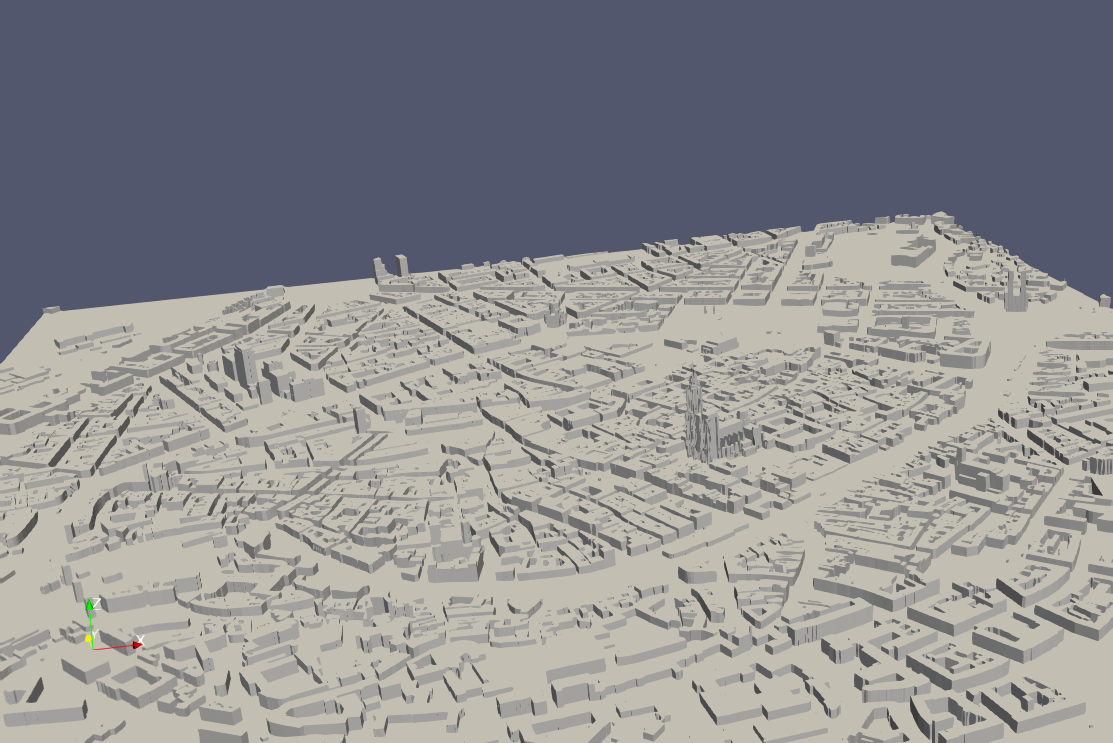
\includegraphics[width=0.75\textwidth]{images/stras_mesh.png}
    \captionsetup{font={scriptsize}}
    \caption{Strasbourg 3D model visualized in ParaView-5.12.0\cite{paraview}}
\end{figure}

However, the software is designed to be easily adaptable to any area.
Here's an example of a 3D model of Manhattan, NYC:

\begin{figure}[H]
    \centering
    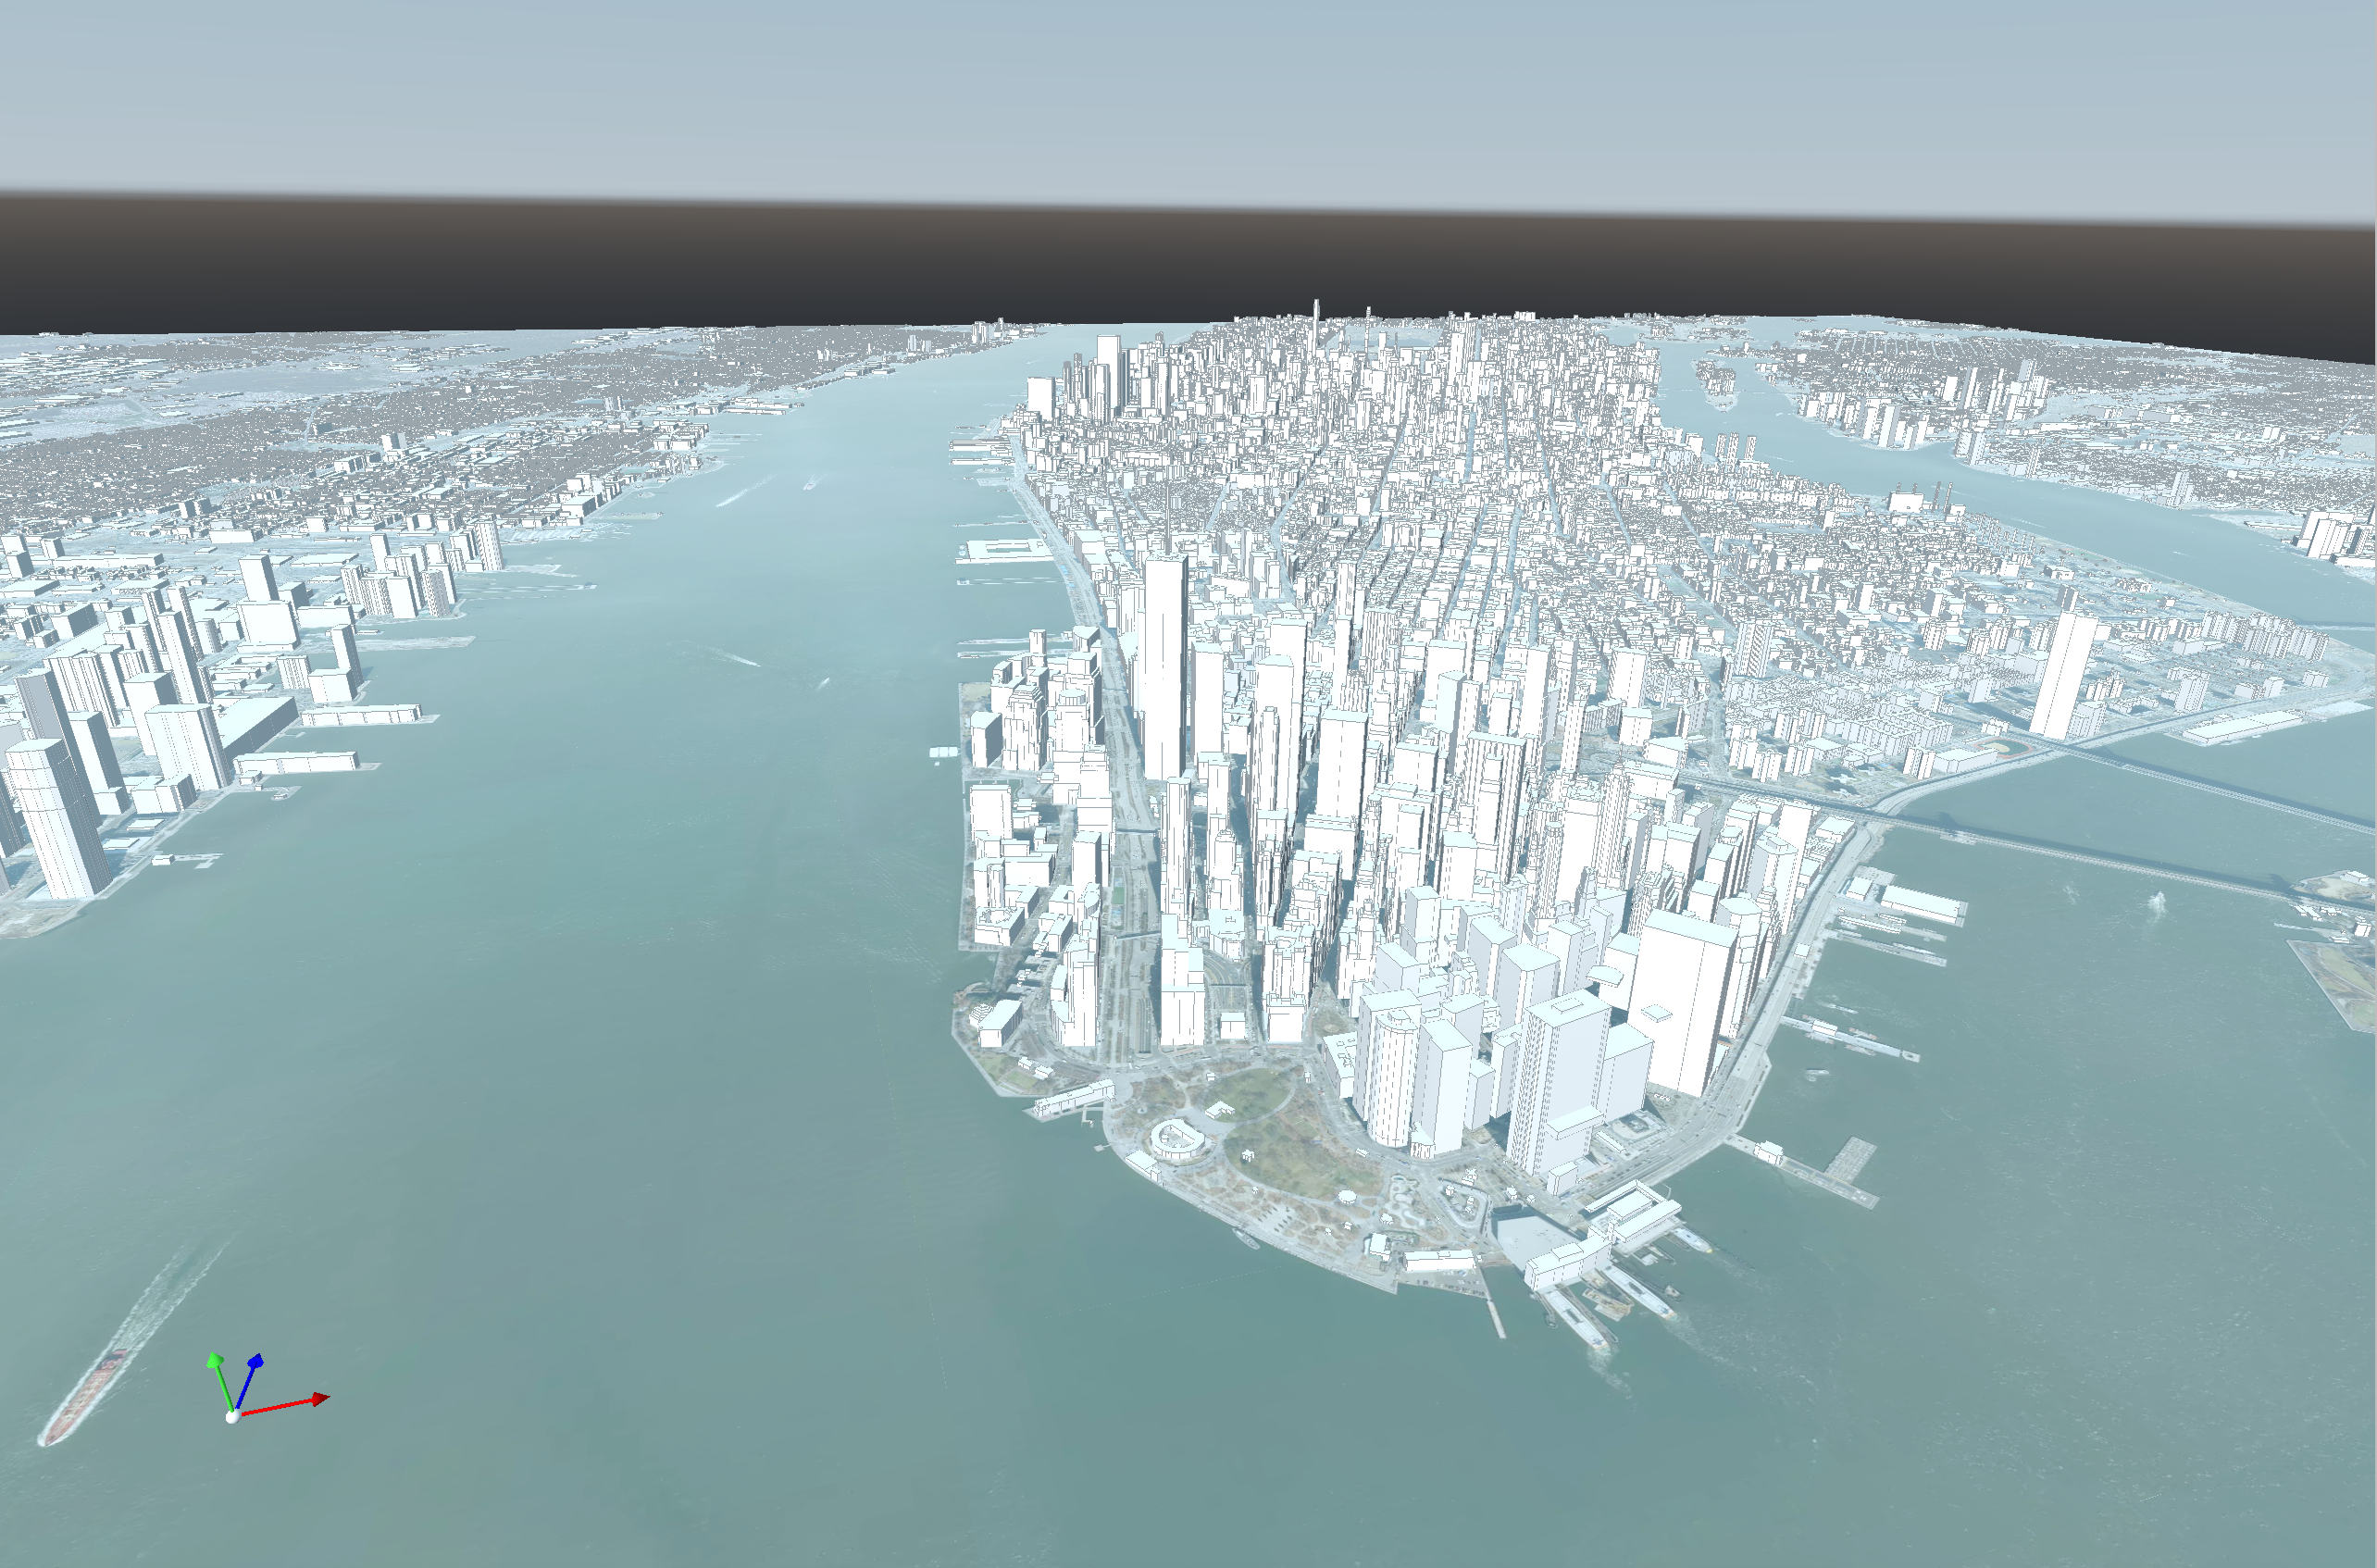
\includegraphics[width=0.75\textwidth]{images/manhattan_mesh.png}
    \captionsetup{font={scriptsize}}
    \caption{Manhattan 3D model}
\end{figure}

\subsection{Main objectives}

\begin{itemize}
    \item Extracting tree data from \texttt{OpenStreetMap}.
    \item Generating 3D tree models using \texttt{CGAL}.
    \item Integrating tree models into the terrain mesh we already have.
    \item Optimizing computational efficiency.
    \item Delivering versions \texttt{V0}, \texttt{V1}, and \texttt{V2} by specified deadlines.
\end{itemize}

\subsection{Software and libraries}
To source our data, we'll utilize the \texttt{Overpass API}\cite{overpass} a
read-only API to query data from \texttt{OpenStreetMap}, alongside
\texttt{cURL}\cite{curl}, a URL transfer library. For geometric modeling, we
will utilize the master \texttt{CGAL} library, available on
GitHub\cite{cgal-master}, known for its efficiency and reliability in geometric
computation.

\subsection{GitHub repository}
We created a \href{https://github.com/master-csmi/2024-m1-vegetation}{GitHub}
repository to manage the project and facilitate collaboration.
The repository contains the project's code, documentation, and resources.
It will be updated regularly to reflect the progress and changes made during
the project's development.

\subsection{Roadmap}
We created a roadmap on GitHub Projects to ensure we meet the deadlines for the
deliverables.
The deadlines are as follows:

\begin{itemize}
    \item \texttt{V0} - 26 March
    \item \texttt{V1} - 23 April
    \item \texttt{V2} - 28 May
\end{itemize}

Here is a brief overview of the main issues:

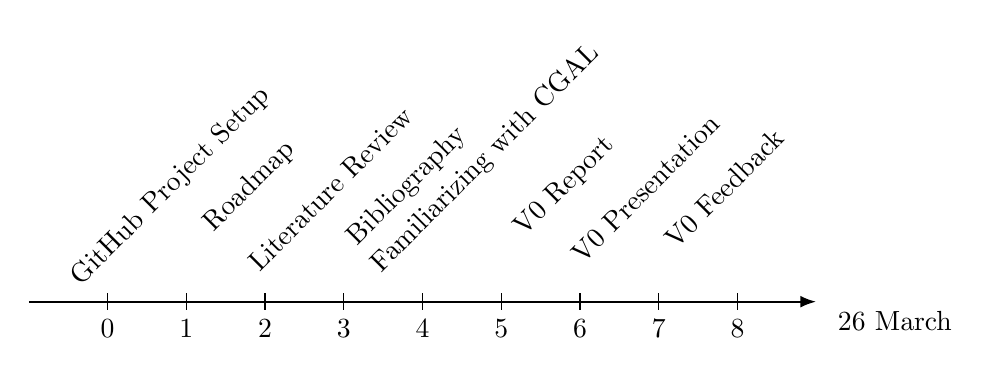
\begin{tikzpicture}

    \draw[thick, -{Latex[length=2mm]}] (0,0) -- (10,0);

    \foreach \x in {1,2,3,4,5,6,7,8,9}
    \draw (\x cm,3pt) -- (\x cm,-3pt);

    \draw (1,0) node[below=3pt] {$ 0 $};
    \draw (2,0) node[below=3pt] {$ 1 $} node[above=30pt, yshift=6pt, rotate=45] {GitHub Project Setup};
    \draw (3,0) node[below=3pt] {$ 2 $} node[above=30pt, yshift=6pt, rotate=45] {Roadmap};
    \draw (4,0) node[below=3pt] {$ 3 $} node[above=30pt, yshift=6pt, rotate=45] {Literature Review};
    \draw (5,0) node[below=3pt] {$ 4 $} node[above=30pt, yshift=6pt, rotate=45] {Bibliography};
    \draw (6,0) node[below=3pt] {$ 5 $} node[above=40pt, yshift=6pt, rotate=45] {Familiarizing with CGAL};
    \draw (7,0) node[below=3pt] {$ 6 $} node[above=30pt, yshift=6pt, rotate=45] {V0 Report};
    \draw (8,0) node[below=3pt] {$ 7 $} node[above=30pt, yshift=6pt, rotate=45] {V0 Presentation};
    \draw (9,0) node[below=3pt] {$ 8 $} node[above=30pt, yshift=6pt, rotate=45] {V0 Feedback};

    \node[below] at (11,0) {26 March};
\end{tikzpicture}

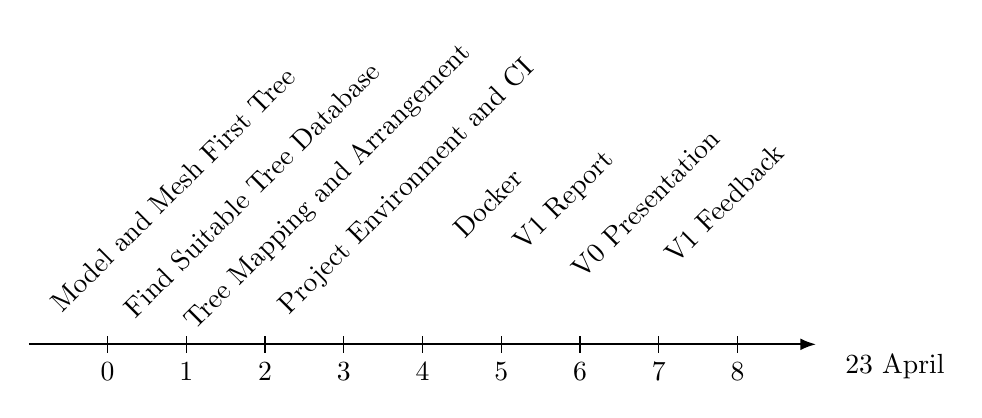
\begin{tikzpicture}

    \draw[thick, -{Latex[length=2mm]}] (0,0) -- (10,0);

    \foreach \x in {1,2,3,4,5,6,7,8,9}
    \draw (\x cm,3pt) -- (\x cm,-3pt);

    \draw (1,0) node[below=3pt] {$ 0 $};
    \draw (2,0) node[below=3pt] {$ 1 $} node[above=45pt, yshift=6pt, rotate=45] {Model and Mesh First Tree};
    \draw (3,0) node[below=3pt] {$ 2 $} node[above=45pt, yshift=6pt, rotate=45] {Find Suitable Tree Database};
    \draw (4,0) node[below=3pt] {$ 3 $} node[above=45pt, yshift=6pt, rotate=45] {Tree Mapping and Arrangement};
    \draw (5,0) node[below=3pt] {$ 4 $} node[above=45pt, yshift=6pt, rotate=45] {Project Environment and CI};
    \draw (6,0) node[below=3pt] {$ 5 $} node[above=40pt, yshift=6pt, rotate=45] {Docker};
    \draw (7,0) node[below=3pt] {$ 6 $} node[above=40pt, yshift=6pt, rotate=45] {V1 Report};
    \draw (8,0) node[below=3pt] {$ 7 $} node[above=40pt, yshift=6pt, rotate=45] {V0 Presentation};
    \draw (9,0) node[below=3pt] {$ 8 $} node[above=40pt, yshift=6pt, rotate=45] {V1 Feedback};

    \node[below] at (11,0) {23 April};
\end{tikzpicture}

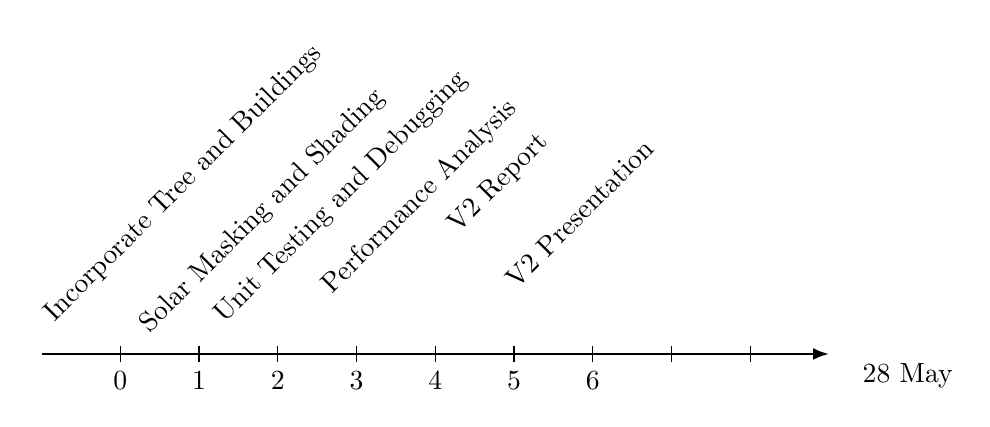
\begin{tikzpicture}

    \draw[thick, -{Latex[length=2mm]}] (0,0) -- (10,0);

    \foreach \x in {1,2,3,4,5,6,7,8,9}
    \draw (\x cm,3pt) -- (\x cm,-3pt);

    \draw (1,0) node[below=3pt] {$ 0 $};
    \draw (2,0) node[below=3pt] {$ 1 $} node[above=50pt, yshift=6pt, rotate=45] {Incorporate Tree and Buildings};
    \draw (3,0) node[below=3pt] {$ 2 $} node[above=40pt, yshift=6pt, rotate=45] {Solar Masking and Shading};
    \draw (4,0) node[below=3pt] {$ 3 $} node[above=45pt, yshift=6pt, rotate=45] {Unit Testing and Debugging};
    \draw (5,0) node[below=3pt] {$ 4 $} node[above=45pt, yshift=6pt, rotate=45] {Performance Analysis};
    \draw (6,0) node[below=3pt] {$ 5 $} node[above=50pt, yshift=6pt, rotate=45] {V2 Report};
    \draw (7,0) node[below=3pt] {$ 6 $} node[above=40pt, yshift=6pt, rotate=45] {V2 Presentation};

    \node[below] at (11,0) {28 May};
\end{tikzpicture}

We have adopted the Agile methodology to enhance flexibility and responsiveness
throughout the project.

\newpage

\section{Methodology}

\subsection{Data acquisition}

We will use the \texttt{Overpass API} and \texttt{cURL} to query
\texttt{OpenStreetMap} for all the available tree data within the specified
bounding box:

\begin{lstlisting}[language=C++]
curl_easy_setopt(curl, CURLOPT_URL,
                "http://overpass-api.de/api/interpreter");

// Set the Overpass query with the bounding box
std::string query =
    "[out:json]; (node(" + bbox + ")[\"natural\"=\"tree\"];); out;";

    std::cout << "Query: " << query << std::endl;
\end{lstlisting}

The \texttt{http://overpass-api.de/api/interpreter} endpoint interprets and
executes the \texttt{Overpass QL}\cite{overpass-ql} queries, retrieving
specific parts of the \texttt{OpenStreetMap} data. In this case, the query
fetches all nodes within the given bounding box tagged as \texttt{natural=tree}.

A \textit{config.json} file is available for the user to specify the area of
interest and other parameters:

\begin{lstlisting}[language=json]
{
    "bbox": "48.5750,7.7394,48.5919,7.7621",
    "origin": "48.583055227464364, 7.748664426560083",
    "altitude": 0,
    "LOD": 3,
    "default_height_range": "3, 6",
    "default_genus": "Platanus",
    "input_building_mesh": "mesh_lod1.stl",
    "output_name": "grande_ile"
}
\end{lstlisting}

Where :
\begin{itemize}
    \item \texttt{bbox}: is the bounding box for the query in the format:
    \subitem (SW latitude, SW longitude, NE latitude, NE longitude)
    \item \texttt{origin}: is the origin of the 3D space in latitude and longitude
    used to convert the GPS coordinates to Cartesian coordinates. It must be the
    same for the terrain mesh and the tree meshes.
    \item \texttt{altitude}: is the z coordinate of the tree base.
    \item \texttt{LOD}: is the level of details of the meshes (0, 1, 2 or 3)
    \item \texttt{default\_height\_range}: is a range used to randomly assign a
    height to trees that do not have one.
    \item \texttt{default\_genus}: is the genus assigned to trees that lack a
    predefined genus.
    \item \texttt{input\_building\_mesh}: is the name of the input file
    representing the terrain mesh.
    \item \texttt{output\_name}: is the base name of the output file
    representing the unions of the tree meshes.
\end{itemize}

The data will be stored in a \textit{.json} file. \\
Here is an example of the query result for one tree:

\begin{lstlisting}[language=json]
{
    "type": "node",
    "id": 10162018740,
    "lat": 48.5850910,
    "lon": 7.7502624,
    "tags": {
        "circumference": "1.47655",
        "diameter_crown": "5",
        "genus": "Platanus",
        "height": "6",
        "leaf_cycle": "deciduous",
        "leaf_type": "broadleaved",
        "natural": "tree",
        "ref": "16401",
        "source": "data.strasbourg.eu - patrimoine_arbore",
        "source:date": "2022-01-02",
        "species": "Platanus acerifolia x",
        "species:wikidata": "Q24853030"
    }
    }
\end{lstlisting}

Sometimes, multiple \texttt{tags} are missing, as shown here:

\begin{lstlisting}[language=json]
{
    "type": "node",
    "id": 4439566691,
    "lat": 48.5839128,
    "lon": 7.7487125,
    "tags": {
      "natural": "tree"
    }
}
\end{lstlisting}

We will primarily use the \texttt{position} of the tree (latitude and
longitude), its \texttt{height}, and the \texttt{genus} (since this data is
more abundant than the species) to generate the 3D tree models.

\newpage

\subsection{Tree library}
We created a library of 13 tree models in \texttt{.stl} format sourced from
the publicly accessible \texttt{SketchUp}\cite{sketchup} 3D Warehouse.

Here is an example of a Ginkgo model that we acquired from \texttt{SketchUp}:

\begin{figure}[H]
    \centering
        \centering
        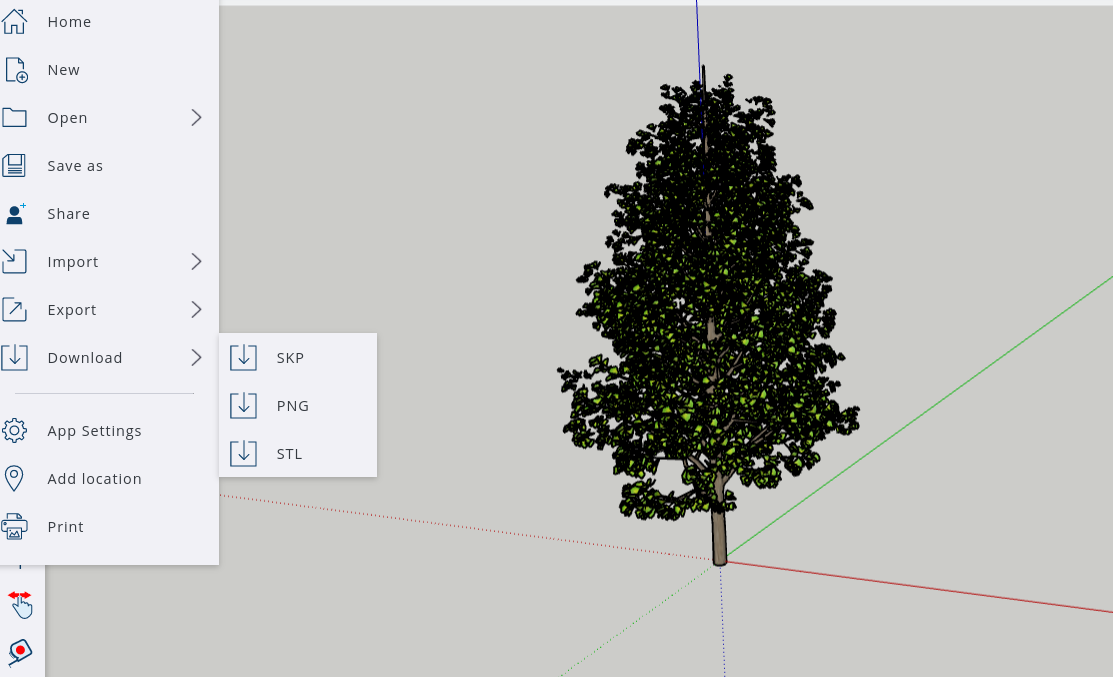
\includegraphics[width=\textwidth]{images/ginkgo_sketchup.png}
        \captionsetup{font={scriptsize}}
        \caption{Mesh of a Ginkgo tree on Sketchup 3D Warehouse}
\end{figure}

\newpage

Below, some of these models visualized using MeshLab\cite{meshlab}:

\begin{figure}[H]
    \centering
    \begin{minipage}{0.24\textwidth}
        \centering
        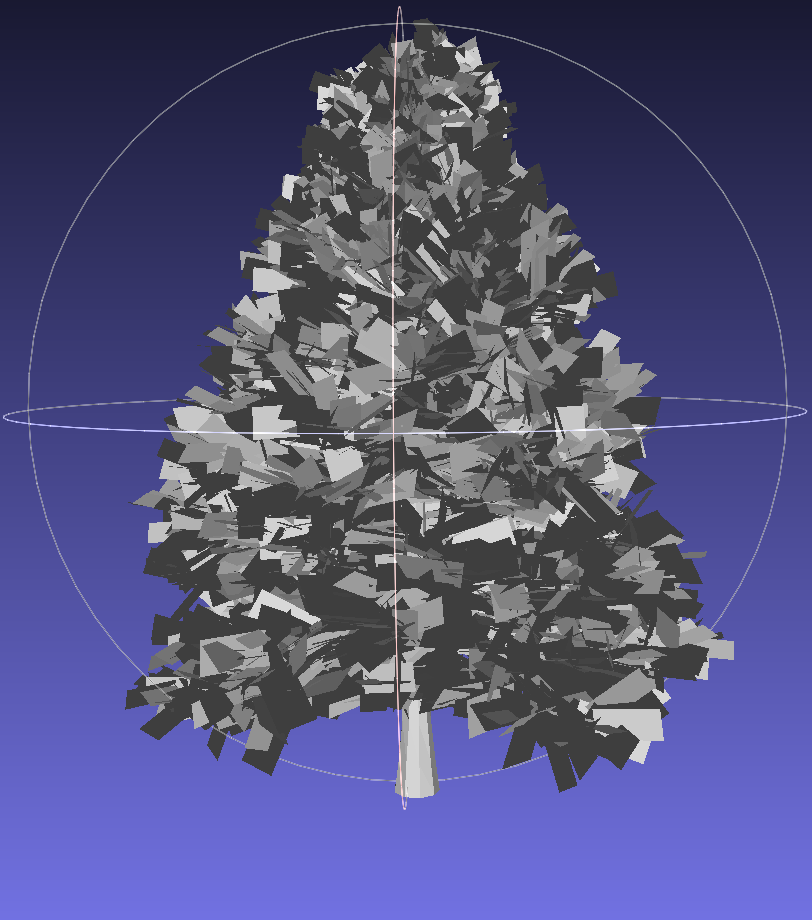
\includegraphics[width=\textwidth]{images/abies.png}
        \captionsetup{font={scriptsize}}
        \caption{Abies}
    \end{minipage}\hfill
    \begin{minipage}{0.24\textwidth}
        \centering
        \includegraphics[width=\textwidth]{images/acer.png}
        \captionsetup{font={scriptsize}}
        \caption{Acer}
    \end{minipage}\hfill
    \begin{minipage}{0.24\textwidth}
        \centering
        \includegraphics[width=\textwidth]{images/aesculus.png}
        \captionsetup{font={scriptsize}}
        \caption{Aesculus}
    \end{minipage}\hfill
    \begin{minipage}{0.24\textwidth}
        \centering
        \includegraphics[width=\textwidth]{images/catalpa.png}
        \captionsetup{font={scriptsize}}
        \caption{Catalpa}
    \end{minipage}
\end{figure}

\begin{figure}[H]
    \centering
    \begin{minipage}{0.24\textwidth}
        \centering
        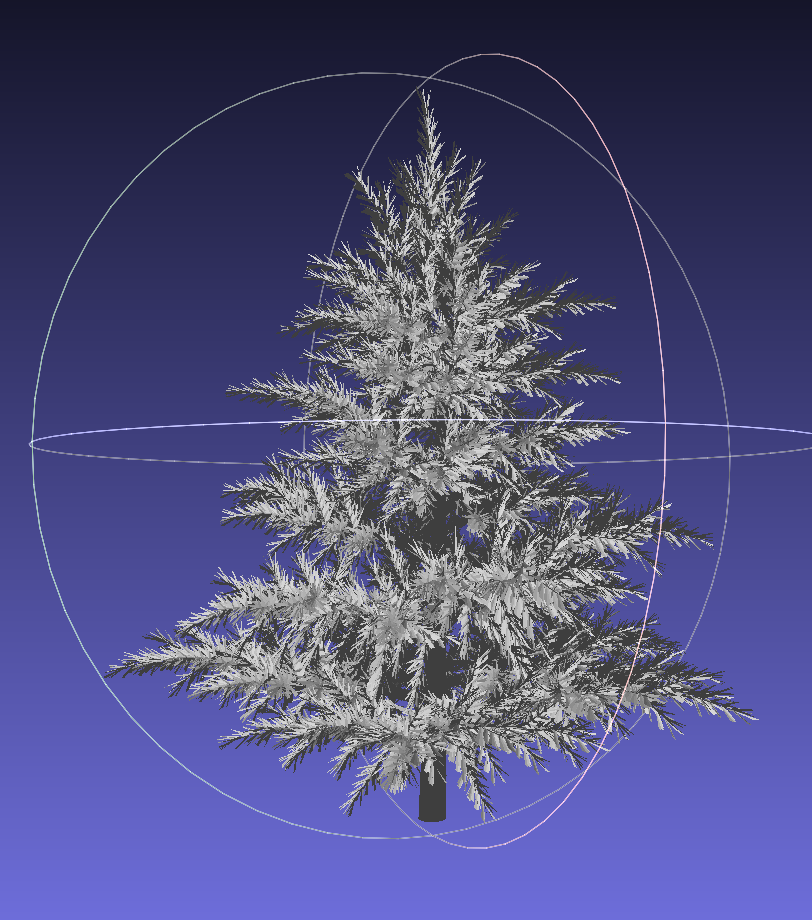
\includegraphics[width=\textwidth]{images/cedrus.png}
        \captionsetup{font={scriptsize}}
        \caption{Cedrus}
    \end{minipage}\hfill
    \begin{minipage}{0.24\textwidth}
        \centering
        \includegraphics[width=\textwidth]{images/liquidanbar.png}
        \captionsetup{font={scriptsize}}
        \caption{Liquidanbar}
    \end{minipage}\hfill
    \begin{minipage}{0.24\textwidth}
        \centering
        \includegraphics[width=\textwidth]{images/platanus.png}
        \captionsetup{font={scriptsize}}
        \caption{Platanus}
    \end{minipage}\hfill
    \begin{minipage}{0.24\textwidth}
        \centering
        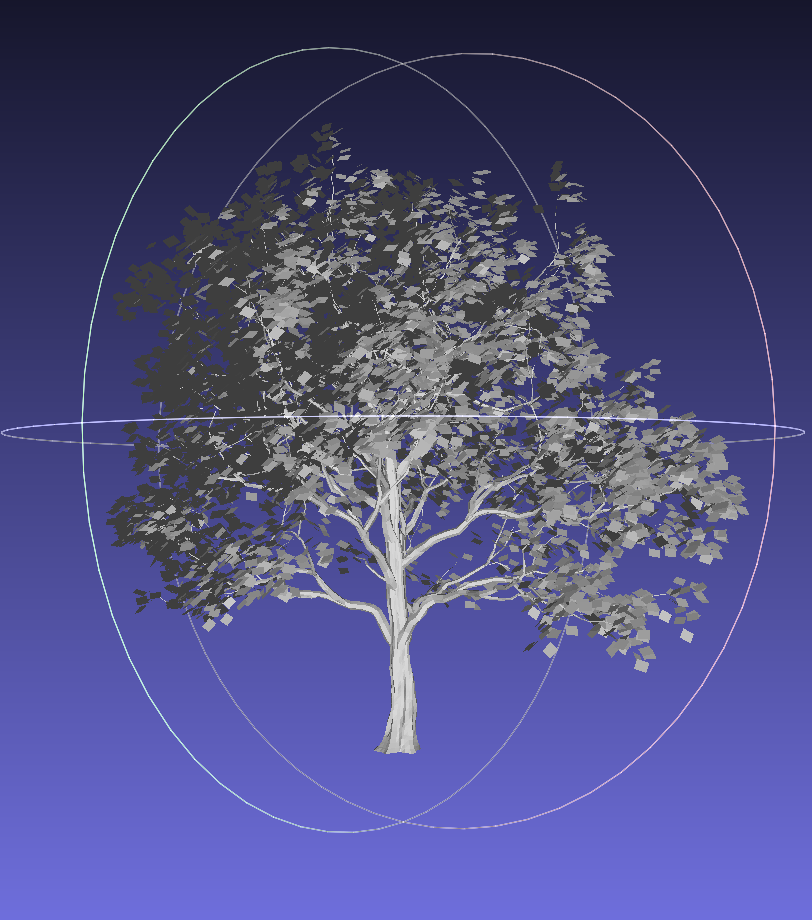
\includegraphics[width=\textwidth]{images/quercus.png}
        \captionsetup{font={scriptsize}}
        \caption{Quercus}
    \end{minipage}
\end{figure}

To ensure the program can handle trees not included in our library, we
categorized an additional 28 genera by matching them to the most similar
models among the 13 trees we have.

\begin{lstlisting}[language=json]
{
    "known_genus": ["Abies",
                    "Acer",
                    "Aesculus",
                     ... ],
    "cedrus_like": [ "Chaemacyparis",
                    "Cupressus",
                     ... ],
    "acer_like": ["Fadus",
                "Metasequoia",
                "Sequoiadendron",
                ... ],
    "liquidambar_like": ["Liriodendron",
                        "Pyrus",
                        "Alnus",
                        ... ],
    "quercus_like": ["Corylus",
                    "Carya",
                    "Fagus",
                    ... ]
}
\end{lstlisting}

\begin{itemize}
    \item \texttt{known\_genus} is a list of the genus for which we have a mesh model.
    \item \texttt{cedrus\_like} is a list of the genus for which the cedrus mesh model will be used.
    \item etc.
\end{itemize}

\newpage

\subsection{Alpha Wrapping}
\begin{figure}[H]
    \centering
        \centering
        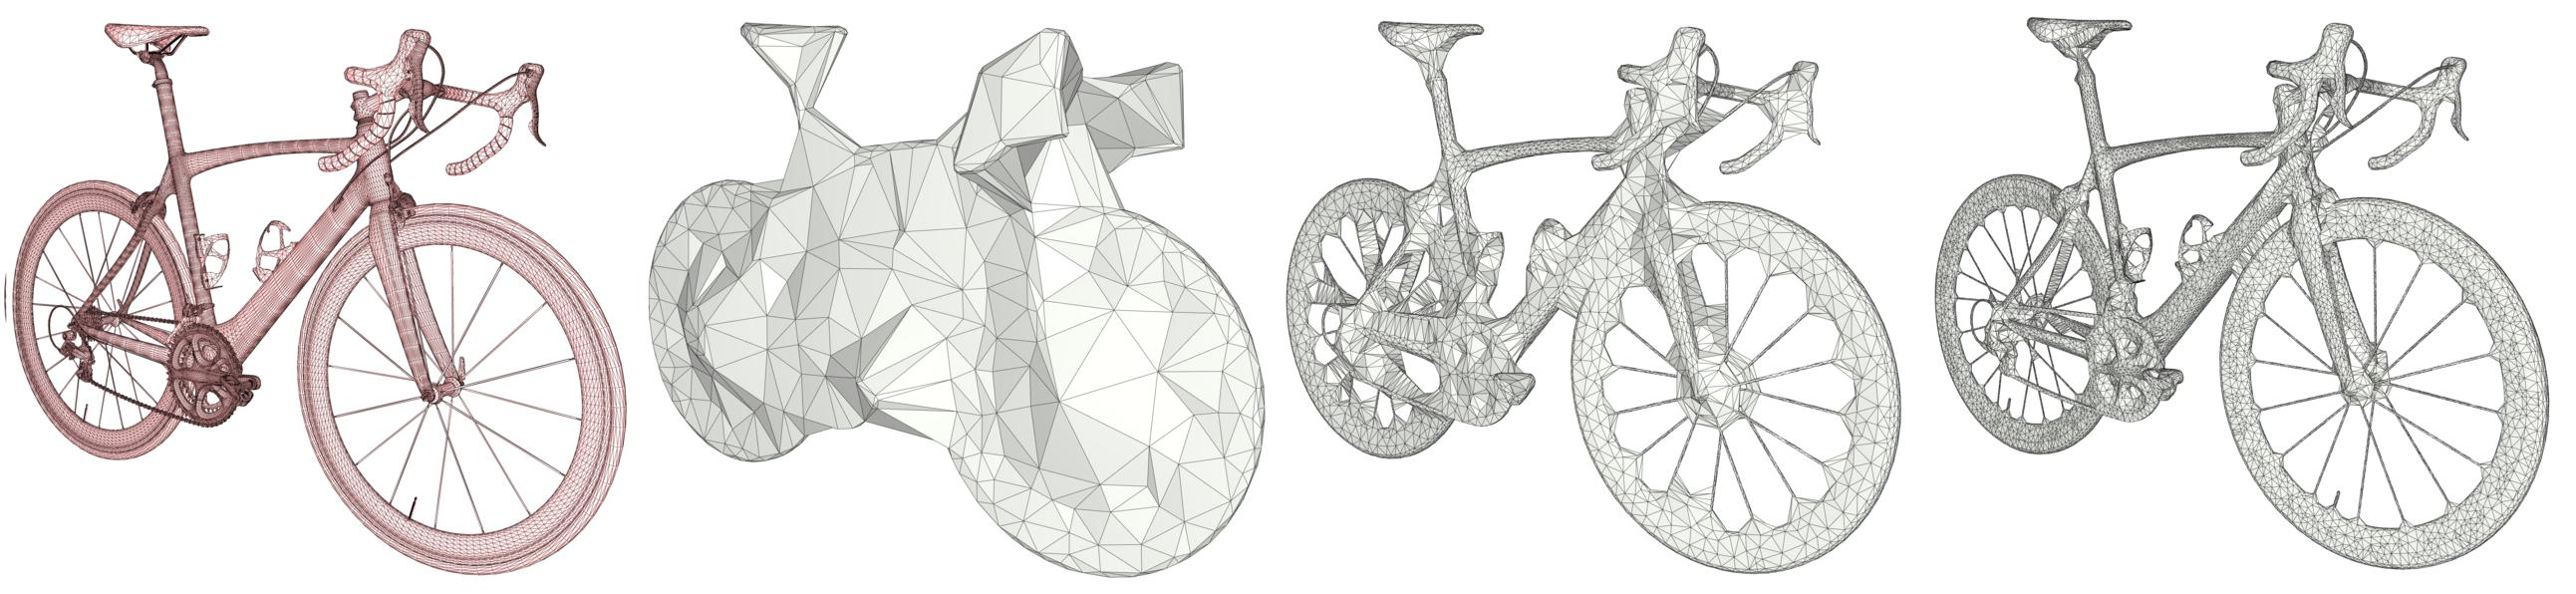
\includegraphics[width=\textwidth]{images/aw3_bike_lod.jpg}
        \captionsetup{font={scriptsize}}
        \caption{Different LOD of the Alpha Wrapping of a bike}
\end{figure}

\textbf{Approach}\\
To enclose a 3D model within a volume, various methods balance runtime and
approximation quality. Simple methods, like bounding boxes, have large errors.
Convex hulls improve quality but remain crude, especially for complex models.
Alpha shapes, a special case of the Delaunay triangulation, offer piecewise-linear
 approximations but struggle with complex input data.

Inspired by alpha shapes, it uses shrink-wrapping, constructing a 3D Delaunay
triangulation and iteratively removing eligible boundary tetrahedra. This process
 refines the triangulation, avoiding inner structures and unnecessary
 computations. This method supports flexible input formats (triangle soups,
 polygon soups, point clouds) and allows trading tightness for mesh complexity.

\textbf{Algorithm Initialization}\\
The algorithm starts by inserting the vertices of a bounding box into a 3D
Delaunay triangulation. In CGAL's 3D Delaunay triangulation, boundary facets
are adjacent to infinite cells tagged as outside, while finite tetrahedra are
tagged inside.

\textbf{Shrink-wrapping}\\
The algorithm traverses from outside to inside cells, using a priority queue of
 Delaunay triangle facets (gates). A gate is alpha-traversable if its circumradius
  exceeds a user-defined alpha. The priority queue, initialized with convex hull
   gates, is sorted by decreasing circumradius. Traversal uses dual Voronoi edges.

When moving from an outside cell \( c_o \) to an inside cell \( c_i \) through
an alpha-traversable facet \( f \):

1. Check for intersections between \( f \)’s dual Voronoi edge and the offset
surface. Insert the first intersection point as a Steiner point into the triangulation.
2. If no intersection but \( c_i \) intersects the input, project \( c_i \)’s
circumcenter onto the offset surface and insert it as a Steiner point.

Newly alpha-traversable gates are added to the queue. If neither criterion is
met, \( c_i \) is tagged outside, and its gates are pushed to the queue. The
process terminates when the queue empties, producing a triangle surface mesh from
 the Delaunay triangulation.

The figure below depicts the steps of the algorithm in 2D.
\begin{figure}[H]
    \centering
        \centering
        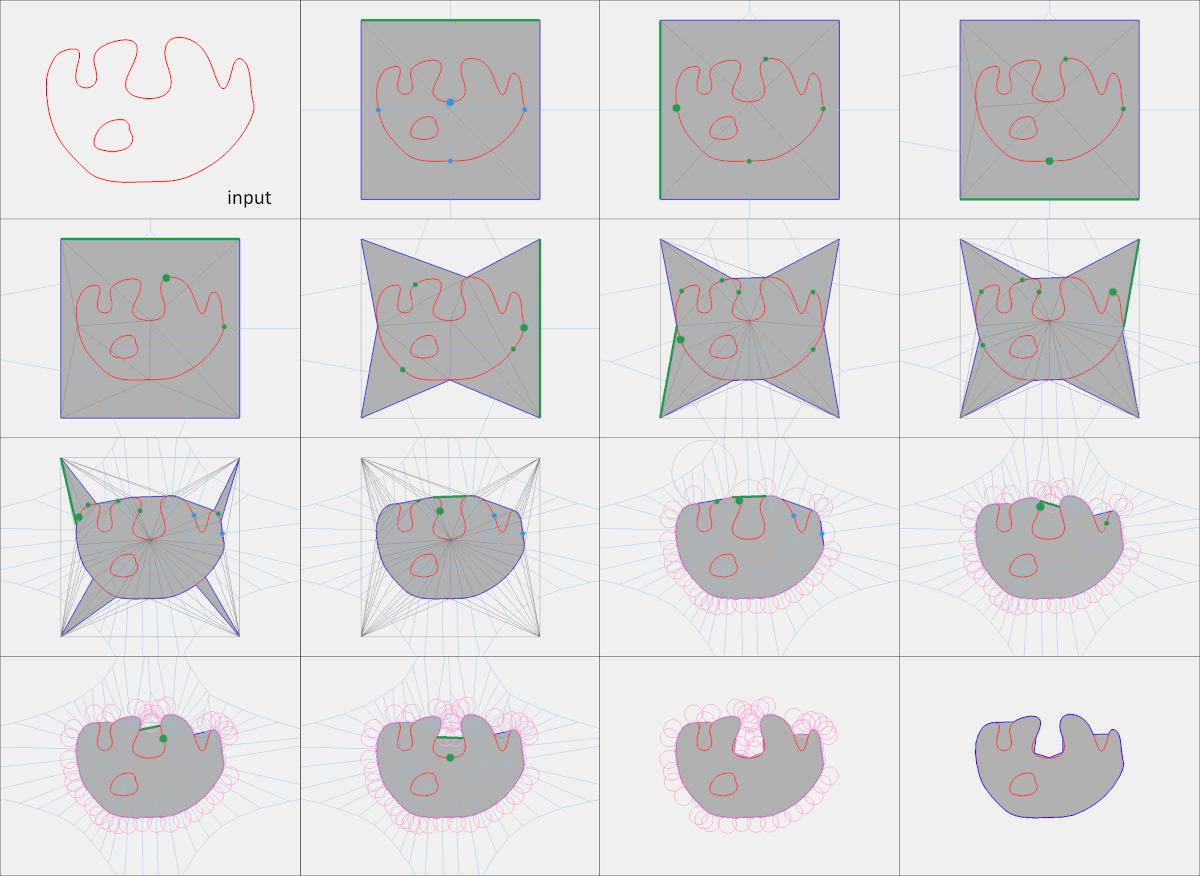
\includegraphics[width=\textwidth]{images/aw3_steps.jpg}
        \captionsetup{font={scriptsize}}
        \caption{Steps of the shrink-wrapping algorithm in 2D. The algorithm
        initializes by inserting the bounding box corners into a Delaunay
        triangulation, tagging finite triangles inside. The current gate (green
        edge) is alpha-traversable. Adjacent triangles are tagged outside if
        they do not intersect the input. If they do, new Steiner points are
        inserted, and traversal resumes. The output edges (dark blue) separate
        inside from outside triangles.
        }
\end{figure}

\textbf{Guarantees} \\
The algorithm guarantees termination and produces a 2-manifold triangulated
surface mesh that encloses the input data. By wrapping from outside to inside
and refining the triangulation as needed, it ensures no intersecting cells are
flagged inside. Steiner points inserted during refinement break necessary cells,
 reducing circumradii and ensuring completion.


\subsection{Tree model generation}
Using the CGAL 3D Alpha Wrapping algorithm, we will generate reference tree
meshes for each level of detail (LOD) from 0 to 3. This pre-processing ensures
that the meshes are readily available in memory, eliminating the need to wrap
each tree model individually during program execution.

A \textit{wrap.cpp} file will be provided to generate the reference meshes.
It can be used as follows:

\begin{lstlisting}[language=bash]
./build/wrap tree_ref/raw_tree/Ginkgo.stl 50 600
\end{lstlisting}

Where 50 is the alpha value and 600 is the offset value.

Additionally, to wrap all the trees in a directory, the \textit{wrap\_all.sh}
script can be used:

\begin{lstlisting}[language=bash]
#!/bin/bash

# Directory containing the raw STL files
INPUT_DIR="tree_ref/raw_tree"

# The alpha value to use for wrapping
ALPHA=100

# Loop through all STL files in the input directory
for input_file in $INPUT_DIR/*.stl; do
	./build/wrap "$input_file" "$ALPHA"
done
\end{lstlisting}

The reference meshes will be used to generate the tree models obtained from
the Overpass query. Each tree model will be generated by scaling the reference
mesh to match the tree's height and position in 3D space. This will be
accomplished using the
\texttt{CGAL Affine Transformation}\cite{cgal_affine_transformation},
which has linear complexity in the number of vertices of the mesh.

\newpage

The alpha parameter for the CGAL wrapper was set as follows for each LOD:

\begin{itemize}
    \item LOD 0: 0.1
    \item LOD 1: 20
    \item LOD 2: 50
    \item LOD 3: 100
\end{itemize}

Here's a table showing the number of faces per tree type and LOD:

\begin{table}[h]
    \centering
    \begin{tabular}{|l|c|c|c|c|}
    \hline
    Tree & LOD 0 & LOD 1 & LOD 2 & LOD 3 \\
    \hline
    Abies & 334 & 920 & 5648 & 35592 \\
    Acer & 326 & 1516 & 10622 & 33606 \\
    Aesculus & 274 & 1068 & 6084 & 28782 \\
    Catalpa & 404 & 946 & 4508 & 19940 \\
    Cedrus & 248 & 974 & 6702 & 27564 \\
    Ginkgo & 332 & 1128 & 7488 & 38258 \\
    Gleditsia & 228 & 1032 & 7506 & 28866 \\
    Liquidambar & 212 & 858 & 5210 & 25146 \\
    Magnolia & 230 & 892 & 7820 & 41150 \\
    Platanus & 286 & 1150 & 7148 & 30670 \\
    Quercus & 274 & 1008 & 8748 & 40426 \\
    Taxus & 370 & 798 & 3644 & 15826 \\
    Tilia & 328 & 1102 & 8104 & 46112 \\
    \hline
    \end{tabular}
    \caption{Number of faces per tree type and LOD}
    \label{tab:my_label}
\end{table}

The offset parameter for the CGAL wrapper was set as 600 for each LOD.

Here are the results for a Ginkgo tree model at each LOD:

\begin{figure}[H]
    \centering
    \begin{minipage}{0.45\textwidth}
        \centering
        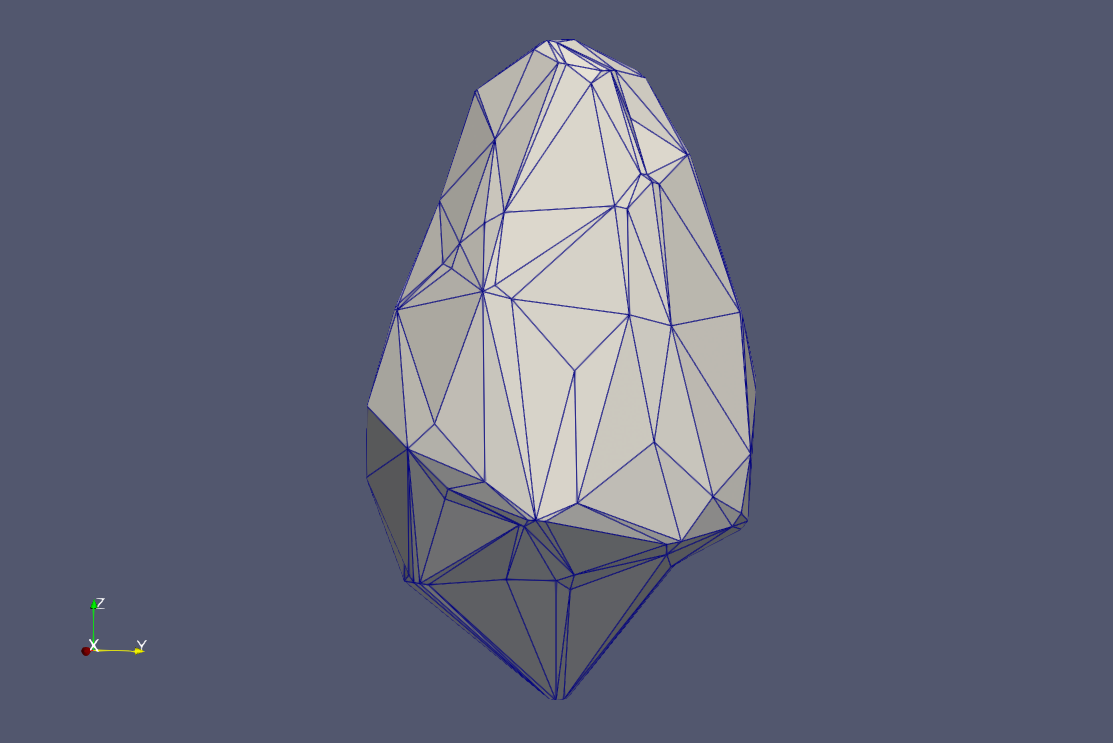
\includegraphics[width=1\textwidth]{images/gingko_lod0.png}
        \captionsetup{font={scriptsize}}
        \caption{Ginkgo lod0}
    \end{minipage}\hfill
    \begin{minipage}{0.45\textwidth}
        \centering
        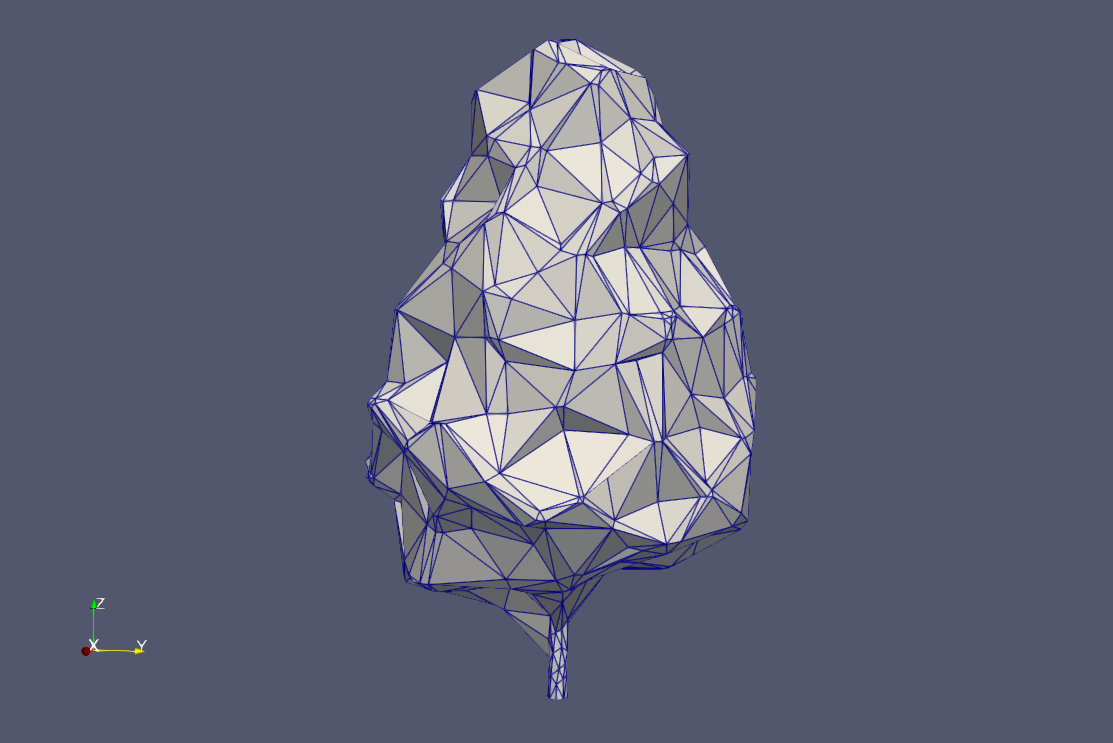
\includegraphics[width=1\textwidth]{images/gingko_lod1.png}
        \captionsetup{font={scriptsize}}
        \caption{Ginkgo lod1}
    \end{minipage}
\end{figure}

\begin{figure}[H]
    \centering
    \begin{minipage}{0.45\textwidth}
        \centering
        \includegraphics[width=1\textwidth]{images/gingko_lod2.png}
        \captionsetup{font={scriptsize}}
        \caption{Ginkgo lod2}
    \end{minipage}\hfill
    \begin{minipage}{0.45\textwidth}
        \centering
        \includegraphics[width=1\textwidth]{images/gingko_lod3.png}
        \captionsetup{font={scriptsize}}
        \caption{Ginkgo lod3}
    \end{minipage}
\end{figure}

The scenario where insufficient data is available for a tree must also be
addressed. Initially, we considered using a k-nearest neighbors
algorithm\cite{k-nn} to determine the tree's metadata (species, height,
leaf density, etc.) based on surrounding trees. However, this approach is
impractical because data is often missing for large areas, such as parks.
Instead, we will assign a random height selected from the
\texttt{default\_height\_range} and a genus specified by
\texttt{default\_genus} in the \textit{config.json} file.

\subsection{Mercator projection}

Generated tree models will be integrated into terrain meshes to create comprehensive
3D urban models. To ensure precise integration into the terrain mesh (especially for large area), the tree models coordinates
(latitude, longitude) will be converted to Cartesian coordinates (x, y) using
a Mercator projection\cite{mercator-proj}.

\begin{figure}[H]
    \centering
    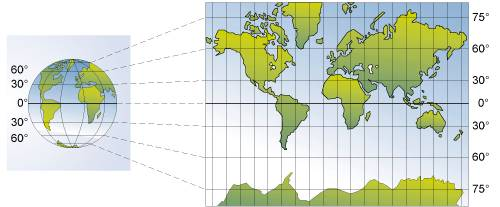
\includegraphics[width=1\textwidth]{images/mercator.jpg}
    \captionsetup{font={scriptsize}}
    \caption{Mercator's projection\cite{img:mercator}}
\end{figure}

This is the most common way to represent the Earth's surface on a plane and has
the advantage of being conformal, meaning that it preserves angles locally (hence
 its usage in sailings). \\
 In a Mercator projection, parallels and meridians are represented by straight
 orthogonal lines, with the equator being the horizontal line placed at the center
  of the map. The other parallels must necessarily be stretched (east-west
  stretching). This stretching is accompanied by a corresponding north-south
  stretching, so that the north-south scale is equal to the east-west scale
  everywhere. \\
  Mathematically, the Mercator projection is defined as follows: if a point on
  the sphere has a latitude $\phi$ and longitude $\lambda$ (with $\lambda_{0}$
  placed at the center of the map), then its projection on the Mercator map will
  have coordinates
  \begin{equation}
    \left\{
    \begin{array}{l}
        x =  \lambda - \lambda_{0} \\
        y =  \ln(\tan(\frac{\pi}{4} + \frac{\phi}{2}))
    \end{array}
    \right.
\end{equation}

To achieve this while taking into account that the Earth is not perfect sphere
we will assume the Earth is a geodesic defined as \texttt{WGS84}\cite{wgs84} and use
the \texttt{WGS84toCartesian}\cite{wgs84_to_cartesian} open source header-only
library to convert the coordinates.

Then the union of all the tree meshed will need to be computed to create a single mesh
and avoid collision between the trees. \\
This will be achieved using the \texttt{corefine and compute}\cite{corefine-compute}
function from the CGAL library.
Another approach could be to use the convex hull of the tree meshes, using the
intersection of the convex hulls to compute the union of the tree meshes.

\subsection{Metrics}
The complexity of the algorithms is a key metric to consider. \\
On each execution of the program, basics metrics will be exported to a text file in
the \texttt{output} directory. \\
These results will be analyzed more thoroughly in the \autoref{sec:Results}.

Example of the result's metrics for \textit{grande\_ile\_LOD1.txt}:

\begin{lstlisting}
Area: 561545 meters
Total number of trees: 409
Number of tree which had no height: 67
Number of tree which had no genus: 27
Number of vertices: 241791
Number of faces: 482686
Time to mesh: 155.965 seconds, (2.59942 minutes)
\end{lstlisting}

\newpage

\section{Implementation}

\subsection{Config class}

This class is designed to store the program's configuration. It will be used to
store the \texttt{bounding box}, the \texttt{level of details}, the \texttt{output name},
the \texttt{default genus}, the \texttt{default height}, the \texttt{origin}, the
\texttt{input building mesh}, and the \texttt{altitude}.

\begin{lstlisting}[language=C++]
class Config {
    private:
        std::string M_bbox;
        int M_LOD;
        std::string M_output_name;
        std::string M_default_genus;
        std::string M_default_height;
        std::string M_origin;
        std::string M_input_building_mesh;
        double M_altitude;

    public:
        Config(std::string const &filename);

        // Ommiting getters and setters

        std::vector<double> bbox_coords() const;
    };

\end{lstlisting}

\subsection{Query function}

The function \texttt{perform\_query} will be used to query the \texttt{Overpass API}
and save the result in a \texttt{.json} file. It will take the bounding box as a
parameter.
The function \texttt{get\_query\_result} will be used to get the result of the query
using the header only library \texttt{nlohmann::json}.

\begin{lstlisting}[language=C++]
void perform_query(std::string bbox);
nlohmann::json get_query_result();
\end{lstlisting}

\subsection{Class tree}

The \texttt{Tree} class will be used to store the tree's metadata and mesh. \\
The function \texttt{computeXY} will be used to convert the latitude and longitude
to Cartesian coordinates using the \texttt{WGS84toCartesian} library. \\
The function \texttt{wrap} will be used to model the tree by scaling and moving
the reference mesh to the correct position in the 3D space. \\
The function \texttt{load\_genus} will be used to load tree genus categories from
the \texttt{trees.json} file. \\
The function \texttt{createTreeFromJson} will be used to create a tree object from
the \texttt{.json} data acquired from the \texttt{Overpass API}. \\
In order to be able to sort trees, the \texttt{operator<} function will be overloaded.


\begin{lstlisting}[language=C++]
using K = CGAL::Exact_predicates_inexact_constructions_kernel;
using Point_3 = K::Point_3;
using Mesh = CGAL::Surface_mesh<Point_3>;

class Tree {
    private:
    long M_id;                    
    double M_lat, M_lon, M_x, M_y; 
    double M_height, M_altitude;   
    double M_circumference, M_diameter_crown; 
    std::string M_genus, M_species, M_season; 
    std::vector<std::string> M_known_genus, M_cedrus_like, M_acer_like,
        M_liquidambar_like, M_quercus_like;
    Mesh M_wrap;                             
    std::vector<Point_3> M_points;           
    std::vector<std::array<int, 3>> M_faces;

    public:
    // Ommiting getters and setters

    void computeXY(double ref_lat, double ref_lon);
    void wrap(int lod);
    void load_genus(const std::string &filename);
};

Tree createTreeFromJson(const nlohmann::json &treeJson);
std::ostream &operator<<(std::ostream &os, const Tree &tree);
bool operator<(const Tree &lhs, const Tree &rhs);
\end{lstlisting}

Each tree model has a CGAL \href{https://doc.cgal.org/latest/Surface_mesh/classCGAL_1_1Surface__mesh.html}{Mesh}
wrapper object that will contain the tree's
mesh and its position in the 3D space.

Scaling and moving the trees into the correct position ended being more complex
than expected.

\begin{lstlisting}[language=C++]
// Calculate centroid of the tree
double centroid_x = 0, centroid_y = 0, centroid_z = 0;
for (const Point_3 &p : points) {
    centroid_x += p.x();
    centroid_y += p.y();
    centroid_z += p.z();
}
centroid_x /= points.size();
centroid_y /= points.size();
centroid_z /= points.size();
Point_3 centroid(centroid_x, centroid_y, centroid_z);

// Calculate bounding box from points
for (const Point_3 &p : points)
    bbox += p.bbox();

scaling_factor_double = M_height / (bbox.zmax() - bbox.zmin());

K::RT scaling_factor(scaling_factor_double); // Convert to exact type

// Find the base of the tree (minimum z-coordinate)
double base_z = std::numeric_limits<double>::max();
for (const auto &p : points) {
    if (p.z() < base_z)
        base_z = p.z();
}

// Create affine transformations
CGAL::Aff_transformation_3<K> translate_to_base(
    CGAL::TRANSLATION, Vector_3(-centroid.x(), -centroid.y(), -base_z));
CGAL::Aff_transformation_3<K> scale(CGAL::SCALING, scaling_factor);
CGAL::Aff_transformation_3<K> translate_back(
    CGAL::TRANSLATION, Vector_3(centroid.x(), centroid.y(), base_z));
CGAL::Aff_transformation_3<K> translate_to_target(CGAL::TRANSLATION,
                                                  Vector_3(M_x, M_y, 0));

// Apply transformations: move to base, scale, move back, move to target
for (auto &p : points) {
    p = translate_to_base.transform(p);   // Move to base
    p = scale.transform(p);               // Scale
    p = translate_back.transform(p);      // Move back to original position
    p = translate_to_target.transform(p); // Move to target position
}
// Clear existing mesh data
M_wrap.clear();

// Add transformed vertices to the mesh and store their descriptors
std::map<Point_3, Mesh::Vertex_index> vertex_map;
for (const auto &p : points) {
    auto v = M_wrap.add_vertex(p);
    // Store the vertex descriptor for the transformed vertex
    vertex_map[p] = v;
}

// Add faces to the mesh
for (const auto &face : faces) {
    // Retrieve vertex descriptors for the face vertices
    Mesh::Vertex_index v0 = vertex_map[points[face[0]]];
    Mesh::Vertex_index v1 = vertex_map[points[face[1]]];
    Mesh::Vertex_index v2 = vertex_map[points[face[2]]];

    // Add the face to the mesh
    M_wrap.add_face(v0, v1, v2);
}
\end{lstlisting}

To ensure the placement was correct we first had to move the tree to the origin
of its bounding box, scale it to the correct height, move it back to its original position
(because scaling it was moving the tree around), and finally move it to the correct position in the 3D space.

Note: To improve tree placement we could also compute the center of mass of a slice
at the base of the tree and use it as its origin

\subsection{Doxygen documentation}

\texttt{Doxygen}\cite{doxygen} documentation is available for the project. Doxygen is a
documentation generator that produces comprehensive reference manuals from
annotated source code.

To generate the documentation, you can use the following command:

\begin{lstlisting}[language=bash]
doxygen Doxyfile
\end{lstlisting}

The documentation will be available in the \texttt{html} directory.\\
You can open it with the browser of your choice, for example with Firefox:

\begin{lstlisting}[language=bash]
firefox html/index.html
\end{lstlisting}

\newpage

\section{Results}
\label{sec:Results}
\subsection{Model integration}

Here is an example of the tree mesh union of Place de la République in Strasbourg
using generic trees and LOD1:

\begin{figure}[H]
        \centering
        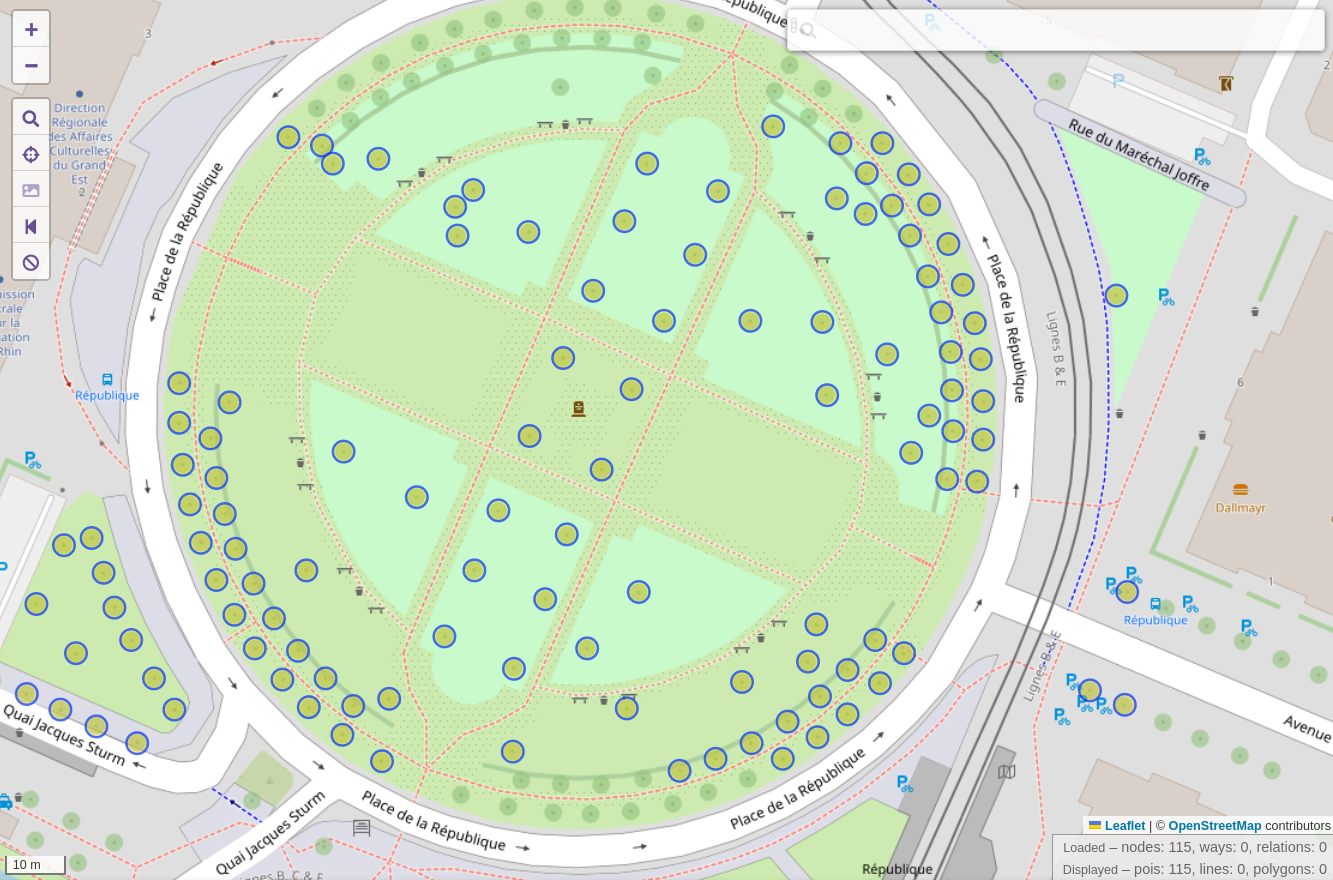
\includegraphics[width=\textwidth]{images/republic_overpassturbo.png}
        \captionsetup{font={scriptsize}}
        \caption{Top view of Place de la République, on the left the mesh generated from the data,
        on the right the overpass data}
\end{figure}

\begin{figure}[H]
        \centering
        \includegraphics[width=\textwidth]{images/republic_lod3.png}
        \captionsetup{font={scriptsize}}
        \caption{3D view of Place de la République}
\end{figure}

The idea is to integrate the tree models into the terrain mesh.

Here is an example of what this integration could look like:

\begin{figure}[H]
    \centering
    \includegraphics[width=0.8\textwidth]{images/strasbourg_mesh_enhanced1.png}
    \captionsetup{font={scriptsize}}
    \caption{Strasbourg 3D model with trees at LOD 0}
\end{figure}

\begin{figure}[H]
    \centering
    \includegraphics[width=0.8\textwidth]{images/strasbourg_mesh_enhanced2.png}
    \captionsetup{font={scriptsize}}
    \caption{Strasbourg 3D model with trees at LOD 0}
\end{figure}

This 2 images are made of 2 distinct meshes, the tree mesh and the building mesh.

\subsection{Complexity and performance analysis}

To assess the complexity and performance of our program, we executed it on
the High-Performance Computing (HPC) cluster Gaya. This cluster consists of a
DELL PowerEdge R7525 head node and six DELL PowerEdge R6525 compute nodes,
providing a total of 768 multi-threaded cores on the compute nodes and 96 cores
on the head node. Gaya offers 150 TB of storage for data and an extremely fast
15 TB NVME scratch space. The head node is equipped with two AMD EPYC 7552
48-Core Processors running at 2.2GHz, totaling 192 virtual cores, and 1024
GB of RAM. Each compute node features two AMD EPYC 7713 64-Core Processors
running at 2GHz, totaling 256 virtual cores, and 512 GB of RAM.
The nodes are interconnected via Broadcom Adv. Dual 10GBASE-T Ethernet and
Mellanox ConnectX-6 Dx Dual Port 100 GbE for MPI communication.

We used four different bounding boxes Strasbourg city center as our test area, all centered at the same point but with
varying sizes:

\begin{figure}[H]
    \centering
    \begin{minipage}{0.45\textwidth}
        \centering
        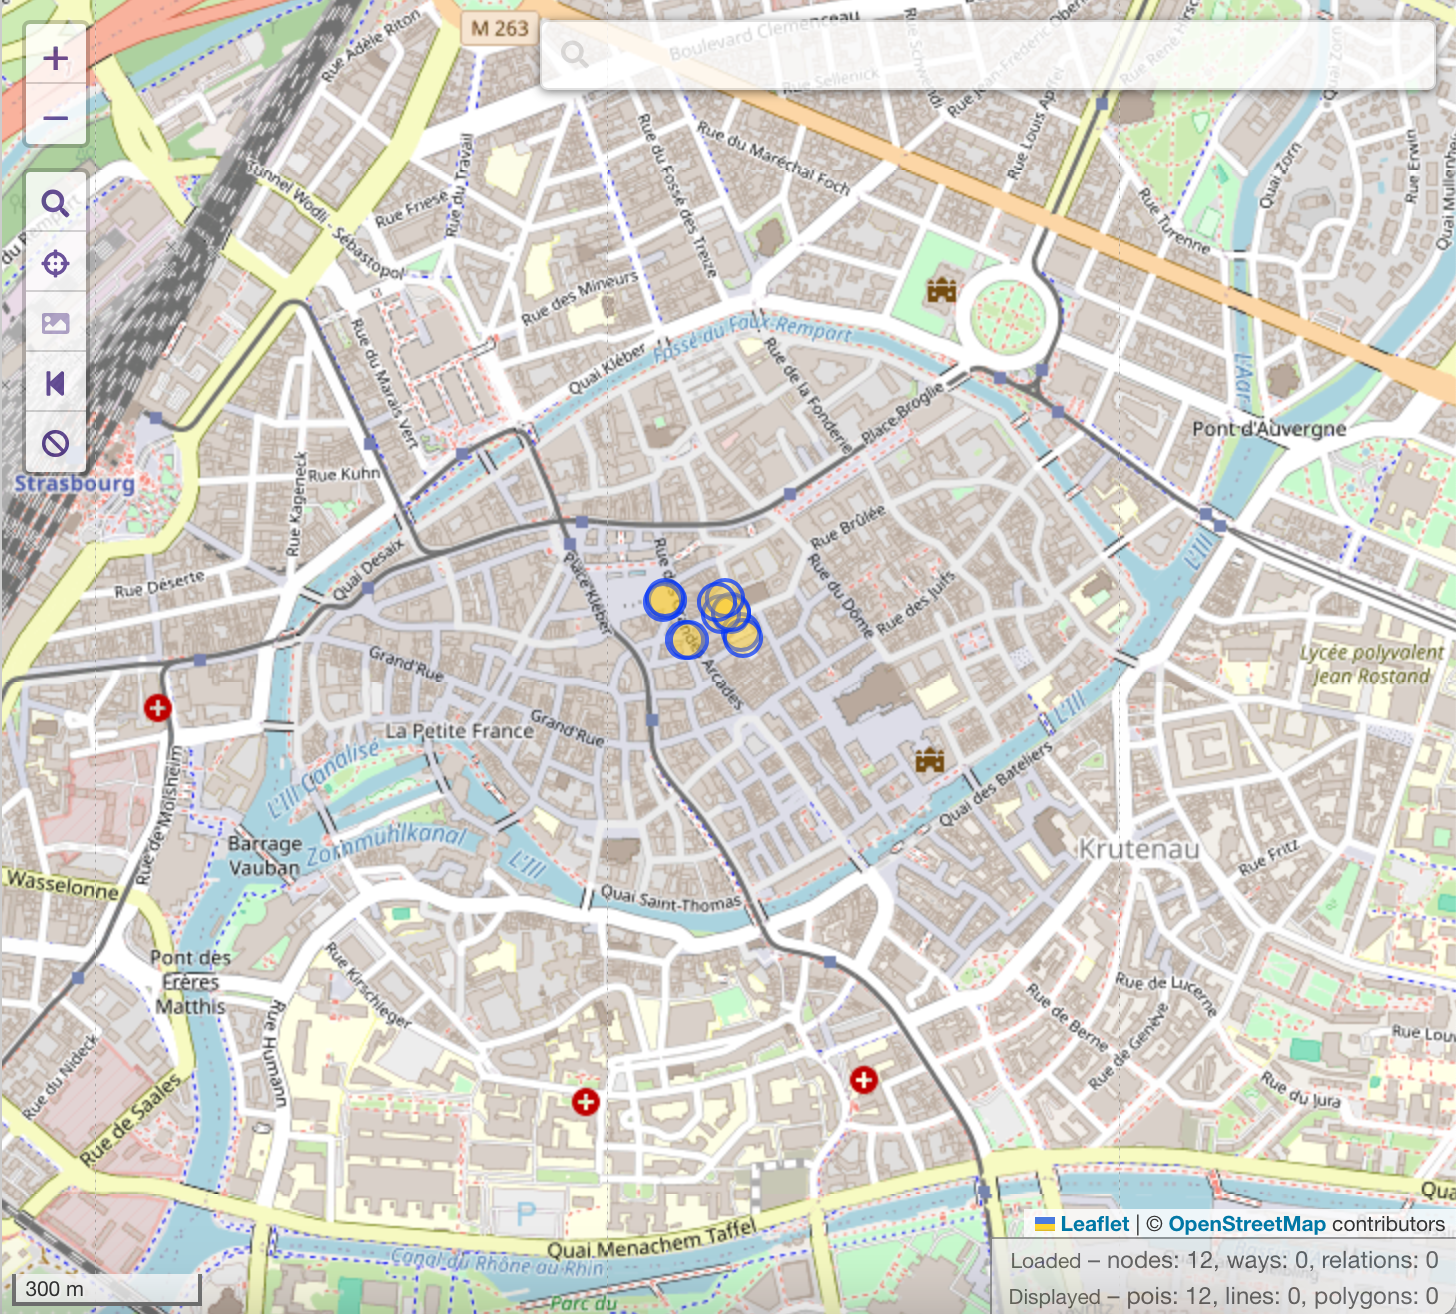
\includegraphics[width=\textwidth]{images/bbox1.png}
        \captionsetup{font={scriptsize}}
        \caption{153.7 m², 12 trees}
    \end{minipage}\hfill
    \begin{minipage}{0.45\textwidth}
        \centering
        \includegraphics[width=\textwidth]{images/bbox2.png}
        \captionsetup{font={scriptsize}}
        \caption{384.0 m², 71 trees}
    \end{minipage}
\end{figure}

\begin{figure}[H]
    \centering
    \begin{minipage}{0.45\textwidth}
        \centering
        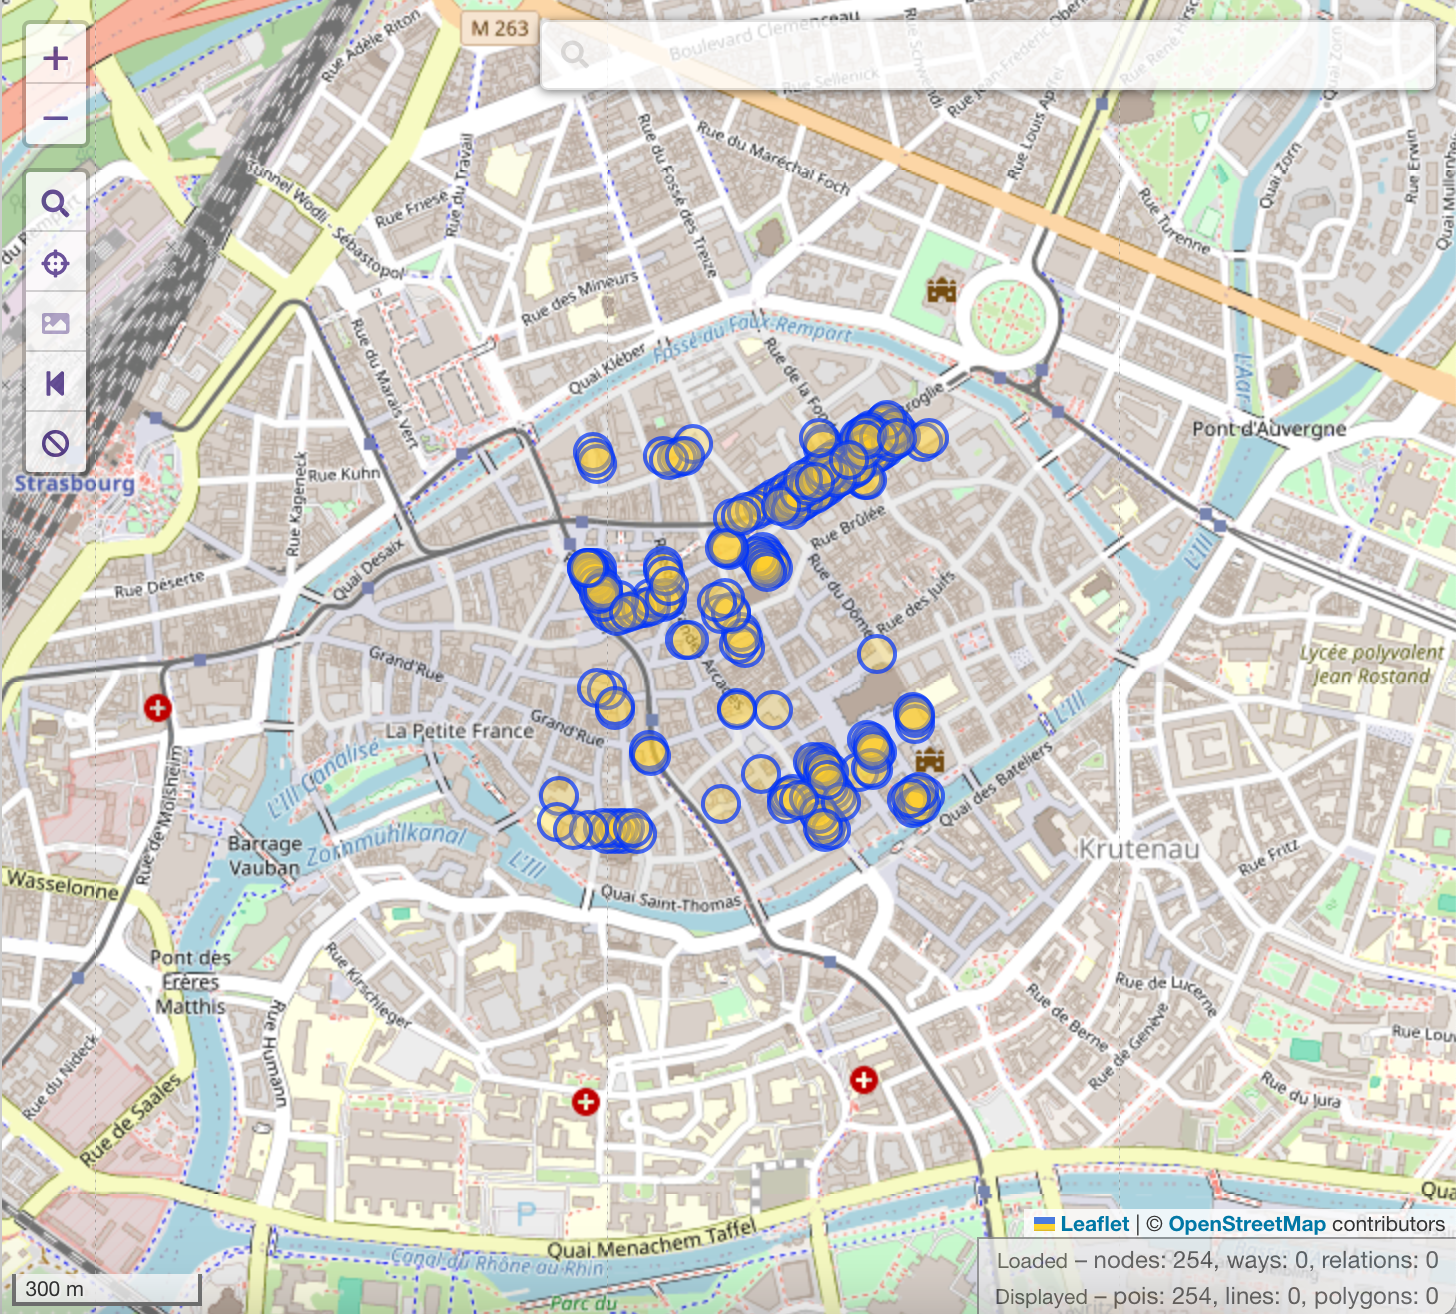
\includegraphics[width=\textwidth]{images/bbox3.png}
        \captionsetup{font={scriptsize}}
        \caption{626.1 m², 254 trees}
    \end{minipage}\hfill
    \begin{minipage}{0.45\textwidth}
        \centering
        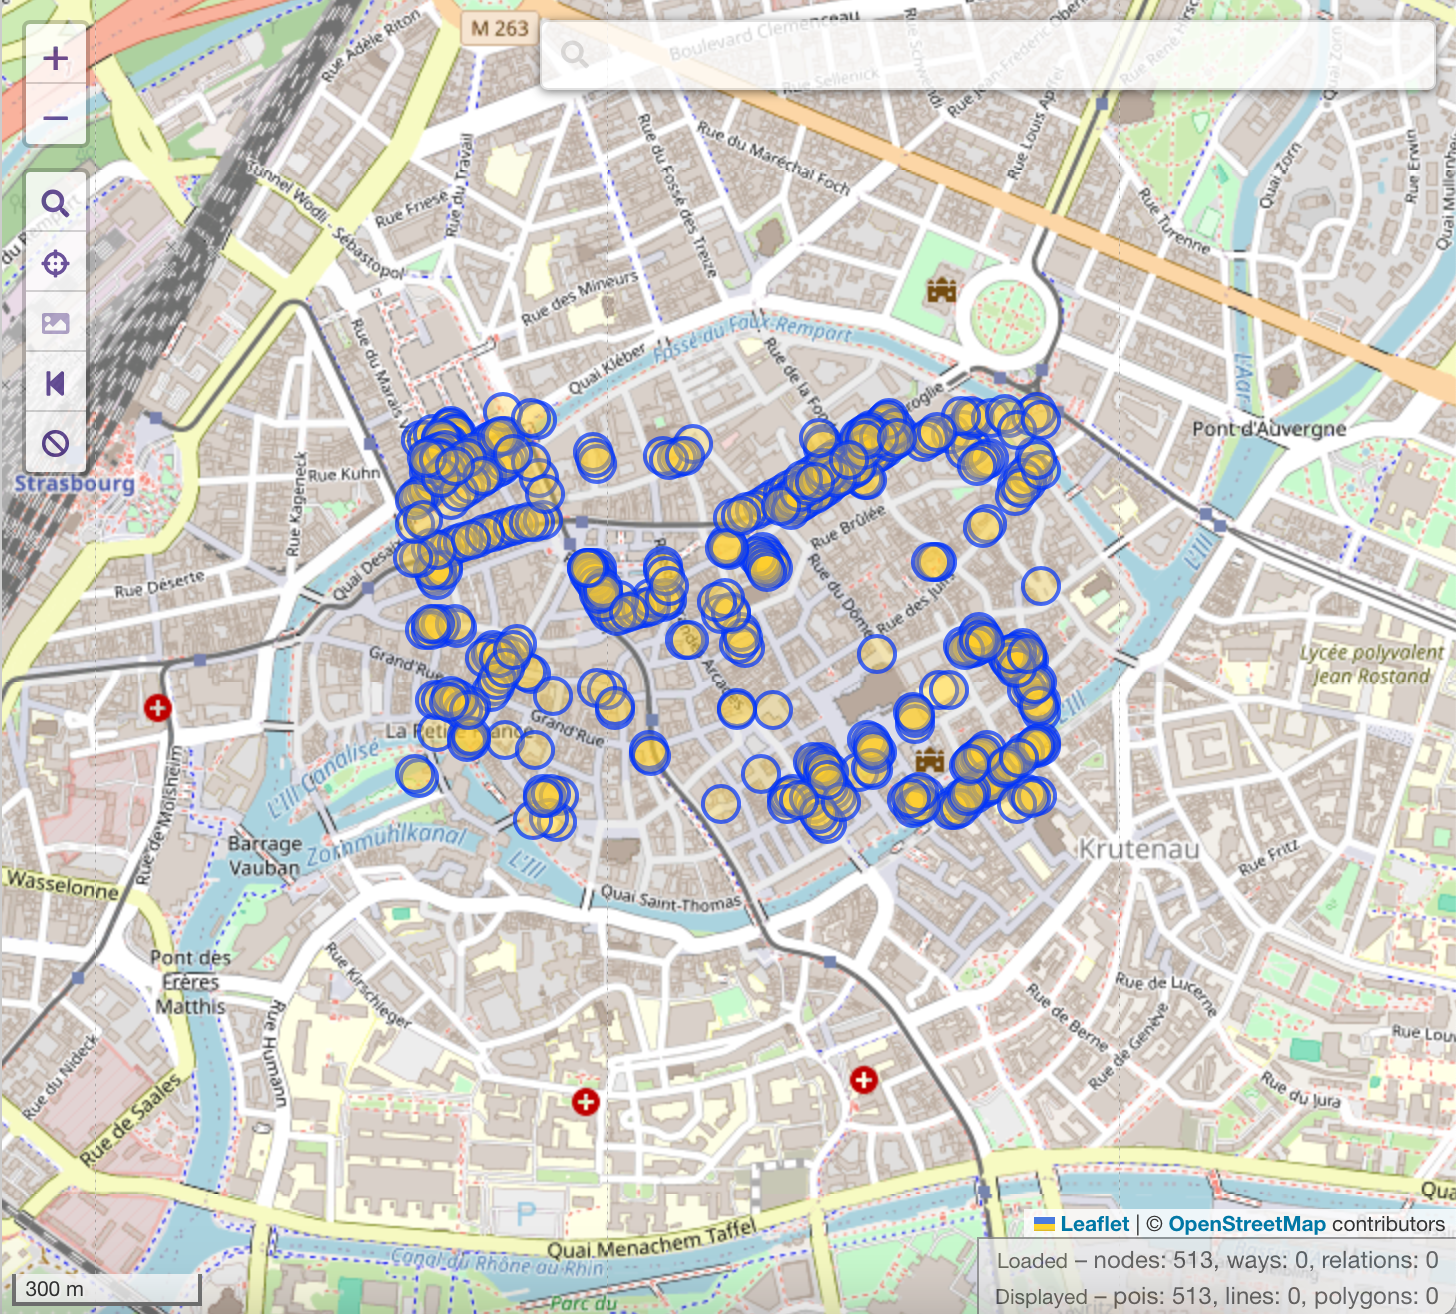
\includegraphics[width=\textwidth]{images/bbox4.png}
        \captionsetup{font={scriptsize}}
        \caption{808.4 m², 513 trees}
    \end{minipage}
\end{figure}


For each bounding box, the program was run for the following Levels of Detail (LODs):

\begin{itemize}
    \item LOD 0
    \item LOD 1
    \item LOD 2
    \item LOD 3
\end{itemize}

\subsubsection{Area and Number of Trees}

Since we're using the area as our main feature (because it is the one we
control when meshing an area), we want to examine how the area (in m²) relates
to the number of trees available.

It is important to note that this relationship highly depends on the
configuration of the environment. In urban settings, trees are not usually
evenly distributed (e.g., avenues, parks, etc.), so we cannot always expect a
linear relationship between the area and the number of trees.

\begin{figure}[H]
    \centering
    \includegraphics[width=1\textwidth]{images/area_vs_trees.png}
    \captionsetup{font={scriptsize}}
\end{figure}

Since the plot is a line on a log-log scale, we can infer that the relationship
between the number of trees and the area (in square meters) follows a power law.

\subsubsection{Impact of the level of detail (LOD)}
The Level of Detail (LOD) we chose has a significant impact. Since we did not
select the LODs in a linear fashion, we aim to examine how the different LODs
are related to the number of faces produced in the meshes.

\begin{figure}[H]
    \centering
    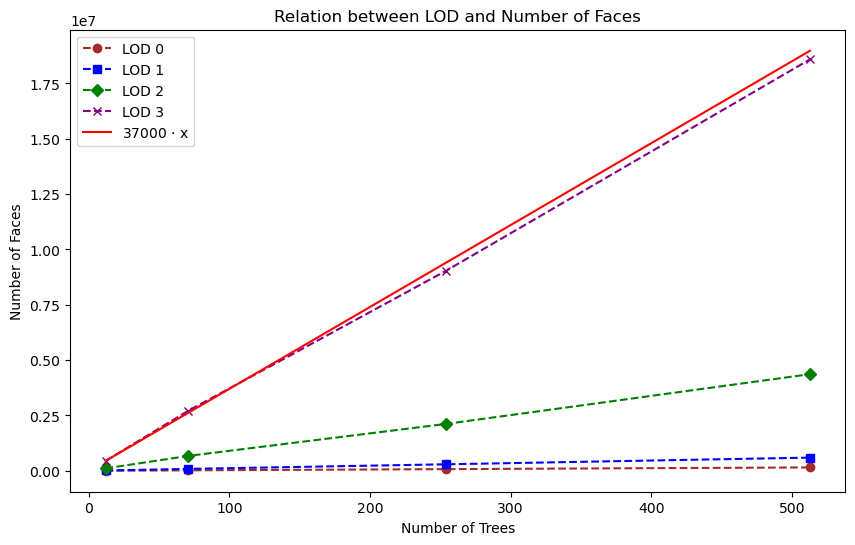
\includegraphics[width=1\textwidth]{images/bench_ntree_nfaces.png}
    \captionsetup{font={scriptsize}}
\end{figure}

The relationship between the number of faces and the Level of Detail (LOD) is
linear. This plot clearly illustrates our choice of LODs, with the last one
being significantly more detailed.

\subsubsection{Execution time}
Finally, we aim to benchmark the time it takes to mesh the area for each Level
of Detail (LOD).

\begin{figure}[H]
    \centering
    \includegraphics[width=1\textwidth]{images/bench_time_ntree_quad.png}
    \captionsetup{font={scriptsize}}
    \caption{Execution time, union of meshes}
\end{figure}

This relationship appears to be quadratic. To confirm this with
greater precision, we would need more data.

\begin{figure}[H]
    \centering
    \includegraphics[width=1\textwidth]{images/bench_time_ntree_linear.png}
    \captionsetup{font={scriptsize}}
    \caption{Execution time, union of triangle soup}
\end{figure}

We can see that making the union using triangle soup instead drastically reduces the
execution time to a linear relationship.



\newpage

\section{Conclusion}

\newpage

\section{Prospects}

\subsection{Account for seasonal changes and leaf fall}
One of the developments of our project is to account for seasonal changes and
leaf fall. Depending on the season, solar rays will penetrate foliage to
varying degrees. To simulate this, we can group leaves into clusters of 5-10
and label them, allowing us to add or remove these clusters in the
configuration file based on the season. To simplify, we can categorize the
seasons into two groups: more leaves for spring and summer, and fewer leaves
for fall and winter.

\subsection{Shading calculations}
Using the \texttt{Feel++}\cite{feel++} library, which specializes in solving
Partial Differential Equations (PDEs) essential for simulating light and shade
on 3D objects, we will simulate ray tracing and shading effects on buildings.
This will help us account for the presence of trees and their impact on urban
microclimates.

\newpage

\section{References}
\bibliographystyle{unsrt}
\bibliography{references}

\end{document}